\chapter{Cross-Lingual Transfer Mechanisms}\label{chp:Transfer}
\section{Knowledge Editing in LLM}
\paragraph{Core Idea:} Cross-lingual knowledge editing in large language models (LLMs) by \citet{wang2023crosslingual} involves editing the model's knowledge in one language and evaluating its impact on another, addressing the unique challenge of maintaining consistent model behavior across linguistic boundaries. The core of cross-lingual knowledge editing lies in its ability to infuse new or updated knowledge into a model in a source language (e.g., English) and assess how these changes affect the model's performance in a target language (e.g., Chinese). This approach is particularly significant given the dynamic nature of knowledge and the continuous evolution of language and facts. For instance, updating a model's understanding from knowing three Honkai-series games to four, after the release of a new game, without full retraining, illustrates the practical utility of knowledge editing in LLMs as shown in Figure \ref{fig: know-edit}.

\begin{figure}[tbh]
	\centering
	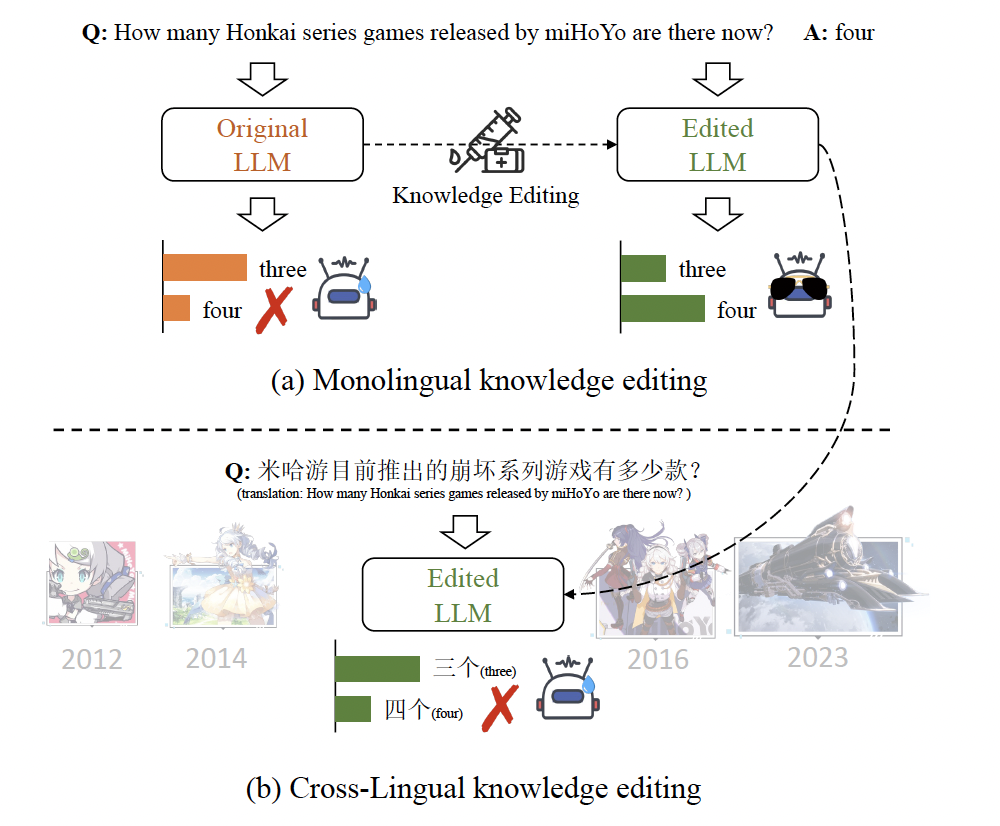
\includegraphics[width=0.75\textwidth]{know-edit}
	\caption[Mono-lingual and Cross-lingual knowledge editing]{Knowledge editing: (a) This shows a language model being updated within the same language. It visually represents the model before and after knowledge editing. For example, before editing, the model might answer ``three" to the question ``How many Honkai series games released by miHoYo are there now?" After editing, to reflect current knowledge, it correctly answers ``four," demonstrating the model's ability to update its information. (b) This depicts the process of editing knowledge in one language (e.g., English) and assessing the update in another language (e.g., Chinese). This shows how the model's response changes from ``three" to ``four" in Chinese after the model has been edited in English, emphasizing the cross-lingual transfer of updated knowledge. (\citet{wang2023crosslingual})}
	\label{fig: know-edit}
\end{figure}

\paragraph{Monolingual Knowledge Editing:} Monolingual knowledge editing focuses on updating a model's knowledge within the same language in which it was originally trained or is primarily operated. This approach is beneficial for quickly integrating new facts or correcting outdated or erroneous information. The typical process involves identifying the specific segments of the model that relate to the outdated or incorrect knowledge and applying targeted updates to these segments. The general approach can be mathematically represented as follows:
\begin{equation}
p'_{\theta}(x) = 
\begin{cases} 
	ye & \text{if } x \in X_e \\
	p_{\theta}(x) & \text{otherwise}
\end{cases}
\end{equation}

where:
\begin{itemize}
	\item \(p_{\theta}(x)\) is the original model's output,
	\item \(p'_{\theta}(x)\) is the updated model's output,
	\item \(X_e\) is the set of inputs for which the knowledge should be updated,
	\item \(ye\) is the new correct output for inputs in \(X_e\).
\end{itemize}

This equation ensures that only the specified aspects of the model are changed, preserving the performance on unrelated tasks or queries.

\paragraph{Cross-Lingual Knowledge Editing:} Cross-lingual knowledge editing extends the concept of monolingual editing by enabling updates made in one language to be reflected in other languages supported by the model. This is particularly challenging due to differences in linguistic structure, semantics, and cultural nuances across languages. The model is first edited in a source language, and the effects of these edits are then assessed in a target language. The mathematical model for cross-lingual knowledge editing involves mapping the edits across languages:

\begin{equation}
p'_{\theta}(x_s) = 
\begin{cases} 
	y_{se} & \text{if } x_s \in X_{se} \\
	p_{\theta}(x_s) & \text{otherwise}
\end{cases}
\end{equation}

\begin{equation}
p'_{\theta}(x_t) = 
\begin{cases} 
	I_t(y_{se}) & \text{if } x_t \in I_t(X_{se}) \\
	p_{\theta}(x_t) & \text{otherwise}
\end{cases}
\end{equation}

where:
\begin{itemize}
	\item \(x_s\) and \(x_t\) represent the input in the source and target languages, respectively,
	\item \(X_{se}\) is the edit scope in the source language,
	\item \(y_{se}\) is the new knowledge in the source language,
	\item \(I_t\) is a function translating source language edits into the target language context.
\end{itemize}

These processes ensure that the model not only learns the new information in the source language but also translates this learning effectively across other languages, thereby maintaining consistency and reliability in multilingual contexts.

\paragraph{Limitations:} While knowledge editing provides a powerful method for updating and refining large language models (LLMs) post-training, it faces several limitations that can affect the efficacy and scope of its application. 
\begin{itemize}
	\item \textbf{Granularity of Edits:} Knowledge editing often requires precise identification of the information needing updates, which can be challenging. The granularity needed for effective edits might not always be achievable, especially in complex models where information is distributed across numerous parameters.
	\item \textbf{Dependency on Edit Quality:} The success of knowledge editing heavily relies on the accuracy and relevance of the edits themselves. Poorly executed or irrelevant edits can lead to model degradation rather than improvement.
	\item \textbf{Translation Inaccuracies:} In cross-lingual settings, translating edits from one language to another can introduce errors due to subtleties in language that are difficult to capture, affecting the model's performance in the target language.
	\item \textbf{Cultural and Contextual Differences:} Edits that are culturally or contextually specific to one language may not be directly applicable or appropriate in another, complicating the transfer of knowledge across languages.
	\item \textbf{Risk of Model Drift:} Frequent and extensive edits risk altering the foundational structures of the model, leading to what is known as model drift where the core capabilities of the model degrade over time.
\end{itemize}

\section{Cross-Lingual Entity Alignment}
\paragraph{Core Idea:} \citet{jiang2023unsupervised} proposed a novel unsupervised method for cross-language entity alignment, which is useful in multilingual knowledge graphs for various applications such as information retrieval and question answering systems. The approach, named Unsupervised Deep Cross-Language Entity Alignment (UDCEA), aims to align semantic entities across different language knowledge graphs without relying on labeled data. The UDCEA approach utilizes a deep learning multi-language encoder combined with a machine translation tool to encode text from knowledge graphs, significantly reducing the dependence on labeled datasets. Unlike traditional methods, which focus on either global or local alignment strategies separately, UDCEA integrates both strategies effectively. It treats the alignment task as a bipartite matching problem and employs a re-exchanging technique to refine the alignment process. This method allows for generating ranked matching results, which are more flexible and useful for various downstream tasks. Figure \ref{fig: know-graph} shows how specific entities (things or concepts) that exist in knowledge graphs of different languages can be aligned or matched to each other.

\begin{figure}[tbh]
	\centering
	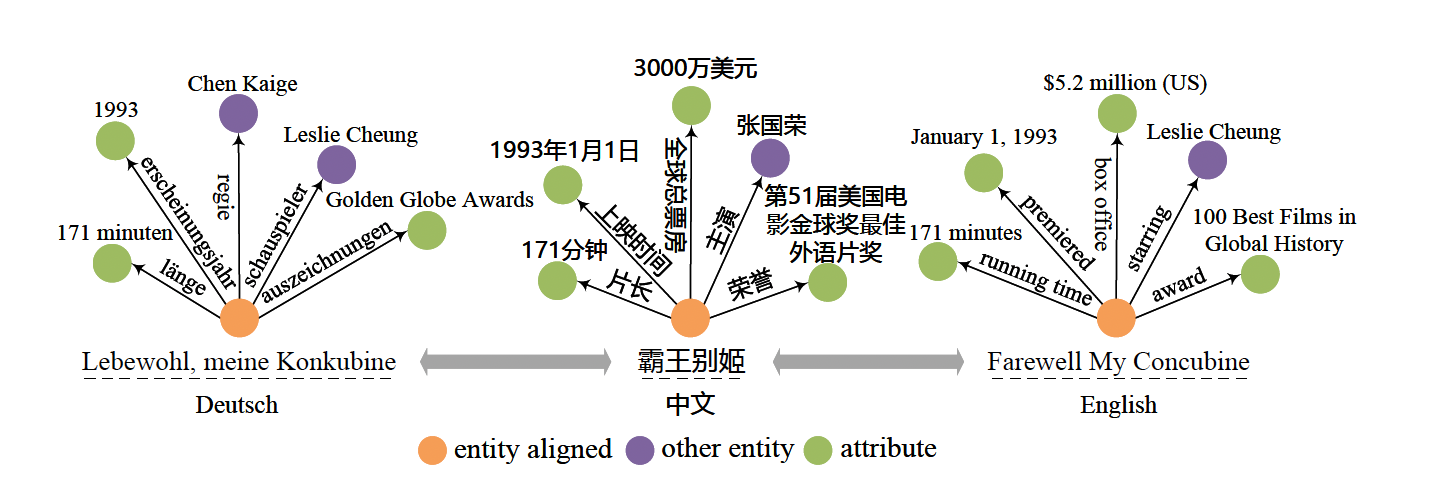
\includegraphics[width=\textwidth]{know-graph}
	\caption[Cross-lingual entity alignment across multiple knowledge graphs]{Cross-lingual entity alignment across multiple knowledge graphs: Orange nodes represent entities that are aligned across different knowledge graphs. An entity can be a thing, like a person, place, or any specific subject. Green nodes are attributes associated with the orange nodes. Attributes provide more details or characteristics about the entities. For example, attributes could be the date of birth of a person, the director of a movie, or the budget of a film. Lines (edges) between nodes show the relationship or connection between an entity and its attributes. This helps to understand how entities are related to their specific characteristics or to other entities. Other nodes (Gray and Yellow) represent other entities and attributes that are part of the knowledge graphs but are not the primary focus for the alignment shown in this figure. (\citet{jiang2023unsupervised})}
	\label{fig: know-graph}
\end{figure}

\paragraph{Feature Embedding:}  The feature embedding module utilizes both machine translation and deep learning encoders to generate embeddings for entities. Let $G_1$ and $G_2$ be two KGs in different languages with entity sets $E_1$ and $E_2$ respectively. The embedding for an entity $e$ in $G_1$ or $G_2$ is computed as follows:

\begin{equation}
	\mathbf{v}_e = \text{Encoder}(\text{Translate}(e))
\end{equation}

Here, $\text{Translate}(\cdot)$ function translates non-English entity descriptions into English, and $\text{Encoder}(\cdot)$ is a pre-trained multilingual model that converts text into a high-dimensional vector space.

\paragraph{Alignment Module:} Once entities are embedded into a vector space, the alignment module aims to find correspondences between entities in $G_1$ and $G_2$. This is formulated as an optimization problem where the distance between supposed matching entities is minimized. The similarity between entities $e_1 \in E_1$ and $e_2 \in E_2$ is given by:

\begin{equation}
	\text{sim}(e_1, e_2) = \mathbf{v}_{e_1} \cdot \mathbf{v}_{e_2}
\end{equation}

A binary variable $x_{e_1e_2}$ is defined which equals 1 if entities $e_1$ and $e_2$ are considered a match and 0 otherwise. The optimization can thus be expressed as:

\begin{equation}
	\max_{x_{e_1e_2} \in \{0,1\}} \sum_{e_1 \in E_1, e_2 \in E_2} x_{e_1e_2} \cdot \text{sim}(e_1, e_2)
\end{equation}
\begin{equation}
	\text{subject to} \quad \sum_{e_2 \in E_2} x_{e_1e_2} \leq 1 \quad \forall e_1 \in E_1
\end{equation}
\begin{equation}
	\sum_{e_1 \in E_1} x_{e_1e_2} \leq 1 \quad \forall e_2 \in E_2
\end{equation}

These constraints ensure that each entity in $G_1$ is matched to at most one entity in $G_2$ and vice versa.

\paragraph{Limitations:} Despite the advantages of our unsupervised deep cross-language entity alignment method, it is subject to several limitations:

\begin{itemize}
	\item \textbf{Dependency on Translation Quality:} The performance of the method heavily depends on the quality of machine translation. Errors in translation can lead to incorrect embeddings and consequently, poor entity alignment.
	
	\item \textbf{Scalability Issues:} The method may not scale well to very large knowledge graphs due to increased computational demands, particularly in the optimization phase. This limitation poses challenges in handling datasets with a large number of entities.
	
	\item \textbf{Difficulty with Polysemous Entities:} Entities that have multiple meanings or are context-dependent can be a challenge. The method may align such entities incorrectly if their textual descriptions in the knowledge graphs do not distinguish between different contexts or meanings.
	
\end{itemize}



